% =====================================================================
\section{Matching a Vector Field (or Gradient) to Its Plot}\label{ch:idfields}
% =====================================================================

\begin{keybox}{The 6-step checklist for $\vF(x,y)=\ip{M,N}$}
\begin{enumerate}
\item \textbf{Plug in four test points}: $(1,0)$, $(0,1)$, $(-1,0)$, $(0,-1)$. Draw those four
  arrows in your head and compare. This alone decides most items.
\item \textbf{Constant?} If $M$ and $N$ are numbers, every arrow is the same (parallel, equal
  length).
\item \textbf{What does it depend on?} If $\vF$ depends only on $y$, every \emph{row}
  (horizontal line) of arrows is identical; depending only on $x$, every \emph{column} is.
\item \textbf{Radial or rotating?} $\vF$ parallel to $\ip{x,y}$ means radial (out if the
  multiple is positive, in if negative). $\vF\cdot\ip{x,y}=0$ means tangent to circles,
  i.e.\ rotating: $\ip{-y,x}$ is counterclockwise, $\ip{y,-x}$ clockwise.
\item \textbf{How does the length change?} $\norm{\ip{x,y}}=r$ grows outward;
  $\vx/\norm{\vx}$ has length 1 everywhere; $\vx/\norm{\vx}^3$ has length $1/r^2$ and is huge
  near the origin and tiny far away.
\item \textbf{Where is $\vF=\vzero$?} Solve $M=0,\ N=0$. A field like $\ip{x,y}$ vanishes only
  at the origin; $\ip{y,0}$ vanishes on the whole $x$-axis.
\end{enumerate}
Sign-of-components shortcut: in each quadrant, $M>0$ means the arrow points right, $N>0$ means
it points up.
\end{keybox}

\begin{figure}[H]
  \centering
  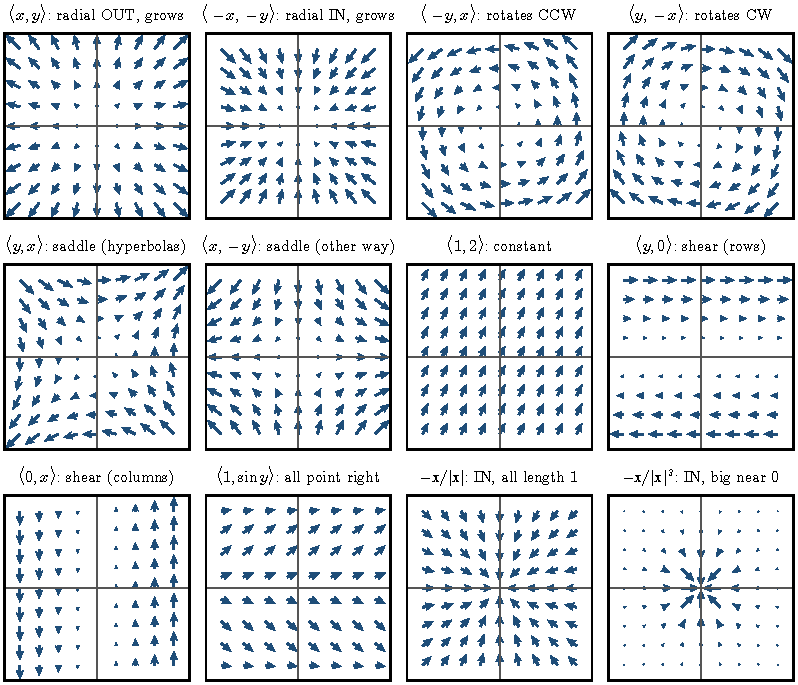
\includegraphics[width=\linewidth]{fields_gallery}
  \caption{The twelve fields that cover almost every matching item. (The last panel is
  capped near the origin so that the arrows stay visible.)}
  \label{fig:fieldsgallery}
\end{figure}

\subsection*{Quick reference: formula $\to$ look}

\begin{center}
\renewcommand{\arraystretch}{1.35}
\begin{tabularx}{\linewidth}{L{0.3\linewidth}Y}
\toprule
\textbf{Field} & \textbf{What the plot looks like}\\
\midrule
$\ip{x,y}$, $c\ip{x,y}$ ($c>0$) & arrows point away from the origin, longer farther out\\
$\ip{-x,-y}$ & arrows point toward the origin, longer farther out\\
$-\vx/\norm{\vx}$ & toward the origin, all the same length\\
$-\vx/\norm{\vx}^3$ (gravity) & toward the origin, very long near it, very short far away\\
$\ip{-y,x}$ & counterclockwise circles, longer farther out\\
$\ip{y,-x}$ & clockwise circles\\
$\ip{-y,x}/(x^2+y^2)$ & counterclockwise circles, \emph{shorter} farther out (vortex)\\
$\ip{y,x}$, $\ip{x,-y}$ & saddle (hyperbolic) pattern: in along one diagonal or axis, out along the other\\
$\ip{a,b}$ & all arrows identical\\
$\ip{y,0}$ & horizontal arrows: right above the $x$-axis, left below, zero on it\\
$\ip{0,x}$ & vertical arrows: up to the right of the $y$-axis, down to the left\\
$\ip{1,\sin y}$ & all point right, tilting up or down in horizontal bands\\
\bottomrule
\end{tabularx}
\end{center}

\subsection*{Vector fields in 3D (slides, Exercise 3)}

Use the same idea: look at what happens on the $z$-axis and as you move away from it.

\begin{figure}[H]
  \centering
  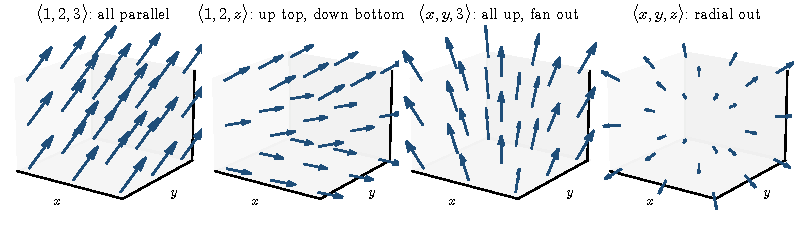
\includegraphics[width=\linewidth]{fields3d_gallery}
  \caption{$\ip{1,2,3}$: constant. $\ip{1,2,z}$: the $z$-component flips sign at $z=0$.
  $\ip{x,y,3}$: always upward, fanning away from the $z$-axis (the slide's answer, C).
  $\ip{x,y,z}$: radial from the origin, so the arrows below $z=0$ point down.}
  \label{fig:fields3d}
\end{figure}

\subsection*{Gradient fields and contour maps}

When the picture is a \emph{contour map} (level curves of $f$), or you must match $f$ to the
plot of $\grad f$:

\begin{keybox}{Rules for gradients on a contour map}
\begin{enumerate}
\item $\grad f$ is \emph{perpendicular} to the level curves.
\item $\grad f$ points toward \emph{higher} values of $f$ (uphill).
\item $\norm{\grad f}$ is \emph{larger} where the level curves are \emph{closer together}.
\item $\Du f>0$ if $\vu$ points uphill (to higher contours), $<0$ if downhill, $=0$ along a contour.
\item Peaks/valleys (closed circles around a point): $\grad f$ points in toward a maximum and out
  from a minimum. At the max/min itself, $\grad f=\vzero$.
\item To match $f$ with a plot of $\grad f$: compute $\grad f$, then use the 6-step checklist.
  A gradient field is conservative, so it \emph{never circulates}: a plot with arrows going
  around in closed loops is \emph{not} a gradient field.
\end{enumerate}
\end{keybox}

\begin{figure}[H]
  \centering
  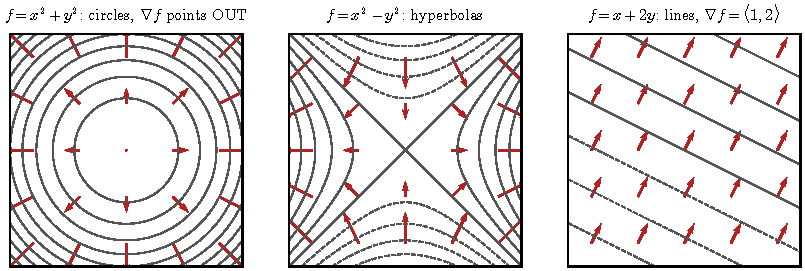
\includegraphics[width=\linewidth]{contours_gradient}
  \caption{Level curves (grey) with gradient vectors (red). The gradient is always
  perpendicular to the level curves and points to larger values. Dashed contours are
  negative levels.}
  \label{fig:contours}
\end{figure}

\subsection*{Level curves to recognise}
\begin{center}
\renewcommand{\arraystretch}{1.35}
\begin{tabularx}{\linewidth}{L{0.36\linewidth}Y}
\toprule
$f(x,y)$ & level curves $f=k$\\
\midrule
$ax+by$ & parallel lines, perpendicular to $\ip{a,b}$\\
$x^2+y^2$ & circles centred at the origin\\
$x^2+2y^2$, $ax^2+by^2$ ($a,b>0$) & ellipses\\
$x^2-y^2$, $xy$ & hyperbolas (plus two crossing lines for $k=0$)\\
$y-x^2$ & parabolas $y=x^2+k$\\
$\sqrt{x^2+y^2}$ vs.\ $x^2+y^2$ & both give circles. For $\sqrt{x^2+y^2}$ (a cone) equally spaced levels give \emph{evenly spaced}
  circles; for $x^2+y^2$ (a paraboloid) the circles get \emph{closer together} farther out\\
\bottomrule
\end{tabularx}
\end{center}
